\input{header}

\AtBeginSubsection[]
{
	\begin{frame}<beamer>
		\frametitle{Outline}
		\tableofcontents[current,currentsubsection]
	\end{frame}
}

\begin{document}

\begin{frame}[allowframebreaks]
  \frametitle{Multi-tape TM $\equiv$ single TM}
  \begin{itemize}
\item Single-tape TM is a special case of multiple-tape TM

\item But how about the other direction?

\item Show single-tape TM can simulate multi-tape TM
\item Fig 3.14

  \end{itemize}  


\begin{center}
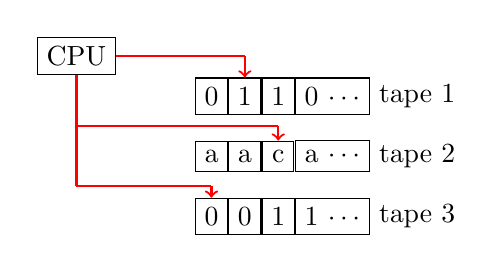
\begin{tikzpicture}[ampersand replacement=\&]
\matrix 
{
  \node[draw](0) {CPU}; \& [1cm]  \& \node(1){} ; \&\&\& \\
  \& \node[draw]{0}; \& \node[draw](a){1}; \& \node[draw]{1}; \& \node[draw]{0 $\cdots$};  \& \node{tape 1};\\
\node(2){} ; \&  \&  \& \node(21){} ; \&\& \\  
\& \node[draw]{a}; \& \node[draw]{a}; \& \node[draw](b){c}; \& \node[draw]{a $\cdots$}; \&  \node{tape 2}; \\
\node(3){} ; \& \node(31){} ; \&  \&  \&\& \\
\& \node[draw](c){0}; \& \node[draw]{0}; \& \node[draw]{1}; \& \node[draw]{1 $\cdots$}; \&  \node{tape 3}; \\
};

\draw [-,red,thick] (0) -- (1.center) ;
\draw [->,red,thick] (1.center) -- (a) ;
\draw [-,red,thick] (0) -- (2.center) ;
\draw [-,red,thick] (2.center) -- (21.center) ;
\draw [->,red,thick] (21.center) -- (b) ;
\draw [-,red,thick] (0) -- (3.center) ;
\draw [-,red,thick] (3.center) -- (31.center) ;
\draw [->,red,thick] (31.center) -- (c) ;
\end{tikzpicture}
\end{center}


\begin{center}
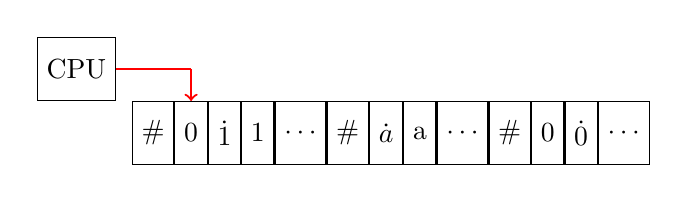
\begin{tikzpicture}[ampersand replacement=\&]
\matrix[nodes={minimum height=8mm}] 
{
  \node[draw](0) {CPU}; \& [0.2cm] \& \node(1){} ; \&\& \&\&\& \&\&\& \&\&\& \\
\& \node[draw]{\#};  \& \node[draw](a){0}; \& \node[draw]{$\dot{1}$}; \& \node[draw]{1}; \& \node[draw]{$\cdots$};
\& \node[draw]{\#};  \& \node[draw]{$\dot{\text{a}}$}; \& \node[draw]{a}; \& \node[draw]{$\cdots$}; 
\& \node[draw]{\#};  \& \node[draw](c){0}; \& \node[draw]{$\dot{0}$}; \& \node[draw]{$\cdots$}; \\
};

\draw [-,red,thick] (0) -- (1.center) ;
\draw [->,red,thick] (1.center) -- (a) ;
\end{tikzpicture}
\end{center}

  \begin{itemize}
\item
  \#: a symbol to separate tapes
\item $\dot{0}$ is used to store the head position of a tape
  
\item $\Gamma$ becomes different:

\item [] $\Gamma$ of original multi-tape TM:
  \begin{equation*}
  \{0,1,a,b,\ldots \}
\end{equation*}
\item [] $\Gamma$ of new single-tape TM:
  \begin{equation*}
  \{0,\dot{0},1,\dot{1},a,\dot{a},b,
\dot{b},\ldots \}
\end{equation*}
\item One multi-tape transition is split to several transitions
\item [] We sequentially conduct them
\item What if the transition is ``move to right (R)'' but we
  see \#?

\item [] $\Rightarrow$ insert a $\sqcup$ and shift things after
\item How to do the shift? An illustration:

  \begin{center}
\begin{tikzpicture}
  \node[state] (q_s) {$q_s$};
  \node[state,above right of=q_s,xshift=1.7cm] (q_0) {$q_0$};
  \node[state,below right of=q_s,xshift=1.7cm] (q_1) {$q_1$};
  \node[state,below right of=q_0,xshift=1.7cm] (q_a) {$q_a$};    
  \path (q_s) edge[above] node{
       $0 \rightarrow \sqcup,$ R
     } (q_0);
  \path (q_s) edge[below] node{
       $1 \rightarrow \sqcup,$ R
  } (q_1);
  \path (q_0) edge[bend right=15, left] node{
       $1 \rightarrow 0,$ R
     } (q_1);
  \path (q_0) edge[loop right] node{
       $0 \rightarrow $ R
  } (q_0);
  \path (q_1) edge[bend right=15, right] node{
       $0 \rightarrow 1,$ R
  } (q_0);
  \path (q_1) edge[loop right] node{
       $1 \rightarrow $ R
  } (q_1);
  \path (q_0) edge[above] node{
       $\sqcup \rightarrow 0$ 
  } (q_a);
  \path (q_1) edge[below] node{
       $\sqcup \rightarrow 1$ 
  } (q_a);
\end{tikzpicture}
  \end{center}

\item $\Gamma$ is finite. Use states to remember the current
  contents
\end{itemize}\end{frame}

\end{document}

%%% Local Variables:
%%% mode: latex
%%% TeX-master: t
%%% End:

